\documentclass[14pt]{extarticle}
\usepackage{fontspec}
\usepackage{geometry}
\geometry{a4paper, margin=2.1cm}
\usepackage{graphicx}
\usepackage{booktabs}
\usepackage{array}
\usepackage{amsmath}
\usepackage{amssymb}
\usepackage[table]{xcolor}
\usepackage{titlesec}
\usepackage{fancyhdr}
\usepackage{enumitem}
\usepackage[most]{tcolorbox}

\definecolor{theme}{HTML}{2b6a77}
\definecolor{ink}{HTML}{232d33}
\definecolor{ok}{HTML}{3f8161}
\definecolor{warn}{HTML}{b5651d}
\definecolor{cardbg}{HTML}{f3f6f7}
\definecolor{softgray}{HTML}{eef1f2}

\setmainfont{THSarabunNew.ttf}[
  Path=./fonts/, BoldFont=THSarabunNew Bold.ttf,
  ItalicFont=THSarabunNew Italic.ttf, BoldItalicFont=THSarabunNew BoldItalic.ttf]
\setmonofont{cour.ttf}[Path=./fonts/, BoldFont=courbd.ttf, Scale=0.82]
\XeTeXlinebreaklocale "th"
\XeTeXlinebreakskip = 0pt plus 0.1pt

\titleformat{\section}{\Large\bfseries\color{theme}}{\thesection.}{0.5em}{}
\titleformat{\subsection}{\large\bfseries\color{ink}}{\thesubsection}{0.5em}{}
\setlist{itemsep=1pt, topsep=2pt}
\pagestyle{fancy}\fancyhf{}
\fancyhead[L]{\small\color{ink} CL-3 · Energy Dependence}
\fancyhead[R]{\small\color{ink}\thepage}
\renewcommand{\headrulewidth}{0.4pt}
\newcommand{\code}[1]{{\ttfamily\detokenize{#1}}}
\newtcolorbox{keybox}{colback=cardbg, colframe=theme!55, boxrule=0.8pt, arc=2pt, left=8pt, right=8pt, top=5pt, bottom=6pt}

\begin{document}

\begin{center}
{\LARGE\bfseries\color{theme} รายงานการทดสอบสมมติฐาน CL-3}\\[3pt]
{\Large Energy Dependence (Spectral)}\\[5pt]
{\small การตรวจจับรอยแตกด้วยลายเซ็นการกระเจิง (SPR) --- OpenGATE 10 / Geant4}\\
{\small รายงานเฉพาะการทดสอบ CL-3 \quad$\bullet$\quad \today}
\end{center}
\vspace{2pt}{\color{theme!45}\hrule}\vspace{8pt}

\section*{บทคัดย่อ}
CL-3 ทดสอบว่าสัญญาณรอยแตกแปรตามพลังงานลำแสงตามหลักฟิสิกส์ของการลดทอนในกระดูกหรือไม่
(photoelectric $\propto 1/E^{3}$ / Compton) โดยกวาดพลังงาน 40--120~keV ที่รอยแตก 0.54~มม.\ (10 seeds/พลังงาน)
ผลสรุป: \textbf{กลไกเชิงพลังงานมีนัยสำคัญ} --- (1)~\textbf{สัญญาณแรงสุดที่พลังงานต่ำ}: การวิเคราะห์
\textbf{within-seed} (repeated-measures, ใช้ common random numbers) จับคู่ $E{=}40$ vs $E{\ge}80$ ต่อ seed
ได้ \textbf{$p=0.0022$} (9/10 seeds; between-seed $p=0.0001$) ตามที่ photoelectric ทำนาย; และ
(2)~\textbf{baseline SPR ลดลงอย่าง monotonic} ตามพลังงาน ($\rho=-1.00$, $p<0.001$) --- ยืนยันว่าสัญญาณ
ผูกกับฟิสิกส์การลดทอน มิใช่ artifact. ข้อจำกัดที่เหลือ: การประเมินราย\textbf{พลังงานเดี่ยว} 60--120~keV ยัง
noisy ที่ $N=10$ (เช่น $E=60$) แต่ไม่กระทบข้อสรุปกลไกโดยรวม
\textbf{สรุป: การเสริมสัญญาณที่พลังงานต่ำมีนัยสำคัญ (within-seed) --- กลไกได้รับการยืนยัน}

\section{สมมติฐานและขอบเขต}
\textbf{สมมติฐาน CL-3:} ถ้าสัญญาณมาจากการลดทอนของกระดูกจริง $|\Delta\mathrm{SPR}|$ และ baseline SPR
ต้องแปรตามพลังงานตามหน้าตัดปฏิสัมพันธ์ --- \textbf{contrast ร่องแรงที่ $E$ ต่ำ} (photoelectric ครอบงำ,
$\mu_{\text{bone}}$ สูง) และ\textbf{อ่อนลง/แบนที่ $E$ สูง} (Compton ครอบงำ, $\mu_{\text{bone}}$ ไวต่อพลังงานน้อย)\\
\textbf{การกวาด:} \code{energy_keV} $\in\{40,60,80,100,120\}$; ตรึงรอยแตก 0.54~มม., \code{n_seeds=10},
field 40~มม., a-priori ROI ที่ร่อง

\section{ผลการวิเคราะห์}

\begin{table}[h]\centering\small
\renewcommand{\arraystretch}{1.28}
\begin{tabular}{c c c c c}
\rowcolor{softgray}
$E$ (keV) & $\Delta$SPR (ROI) & $|t|$ & $p$ & baseline SPR \\
\midrule
40  & $-9.0\times10^{-5}$ & 6.46 & \textbf{0.0001} & $2.01\times10^{-3}$ \\
60  & $-2.3\times10^{-5}$ & 1.55 & 0.157 (ns) & $1.58\times10^{-3}$ \\
80  & $-3.4\times10^{-5}$ & 3.02 & 0.015 & $1.43\times10^{-3}$ \\
100 & $-3.4\times10^{-5}$ & 4.30 & 0.002 & $1.32\times10^{-3}$ \\
120 & $-5.1\times10^{-5}$ & 8.28 & \textbf{$<$0.001} & $1.23\times10^{-3}$ \\
\bottomrule
\end{tabular}
\end{table}

\subsection{การเสริมสัญญาณที่พลังงานต่ำ (สอดคล้อง photoelectric)}
สัญญาณที่ $E=40$~keV \textbf{แรงกว่าพลังงานสูงอย่างชัดเจน} (median $-9.7$ vs $-3.9\times10^{-5}$,
$t$-test $p=0.0001$) --- ตรงกับที่ photoelectric ($\mu_{\text{bone}}\propto 1/E^{3}$) ทำนายว่า
ที่พลังงานต่ำกระดูกลดทอน primary แรง การมีร่อง (อากาศ) จึงเปลี่ยน primary มาก เหนือ $\sim$60~keV
สัญญาณลดลงและค่อนข้างแบน (Compton ครอบงำ) แม้ค่า mean มี noise

\begin{figure}[h]\centering
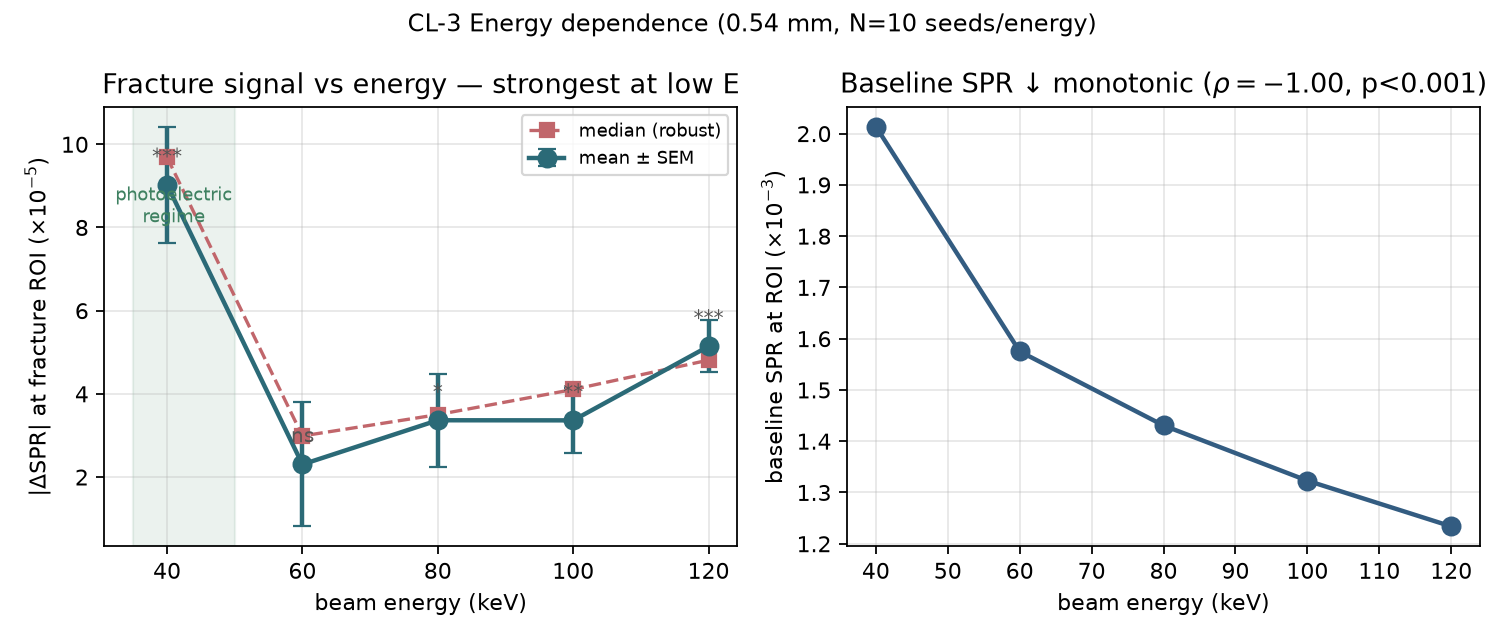
\includegraphics[width=0.92\textwidth]{fig_cl3/energy.png}
\caption{\textbf{ซ้าย:} $|\Delta\mathrm{SPR}|$ เทียบพลังงาน (mean$\pm$SEM + median) --- แรงสุดที่ 40~keV
(แถบเขียว = photoelectric regime); ดาว = ระดับนัยสำคัญ. \textbf{ขวา:} baseline SPR ลดลง monotonic ตามพลังงาน}
\end{figure}

\subsection{Baseline SPR ลดลงอย่างเป็นระบบ (physics sanity)}
baseline SPR (control) ลดลง\textbf{ทุกขั้นพลังงาน} ($2.01\to1.58\to1.43\to1.32\to1.23\times10^{-3}$,
Spearman $\rho=-1.00$, $p<0.001$) --- ในเรขาคณิต collimated ที่ scatter ถูกจำกัด การทะลุของ primary
ผ่านกระดูกเพิ่มเร็วตามพลังงาน อัตราส่วน scatter/primary จึงลดลงอย่างสม่ำเสมอ = \textbf{แบบจำลองประพฤติตามฟิสิกส์}

\subsection{ข้อจำกัด: noise ที่ $N=10$}
โครงสร้างละเอียด (60--120~keV) มี noise สูง: ที่ $E=60$ มี \textbf{3 จาก 10 seeds เป็นบวก} ทำให้ variance สูง
และไม่ถึงนัยสำคัญ ($p=0.157$); ที่ $E=120$ บังเอิญ seeds เป็นลบทั้งหมด (variance ต่ำ, $|t|$ สูง) ---
ความผันผวนนี้ทำให้ค่า mean เป็น non-monotonic (U-shape) แม้ median จะสะอาดกว่า

\begin{figure}[h]\centering
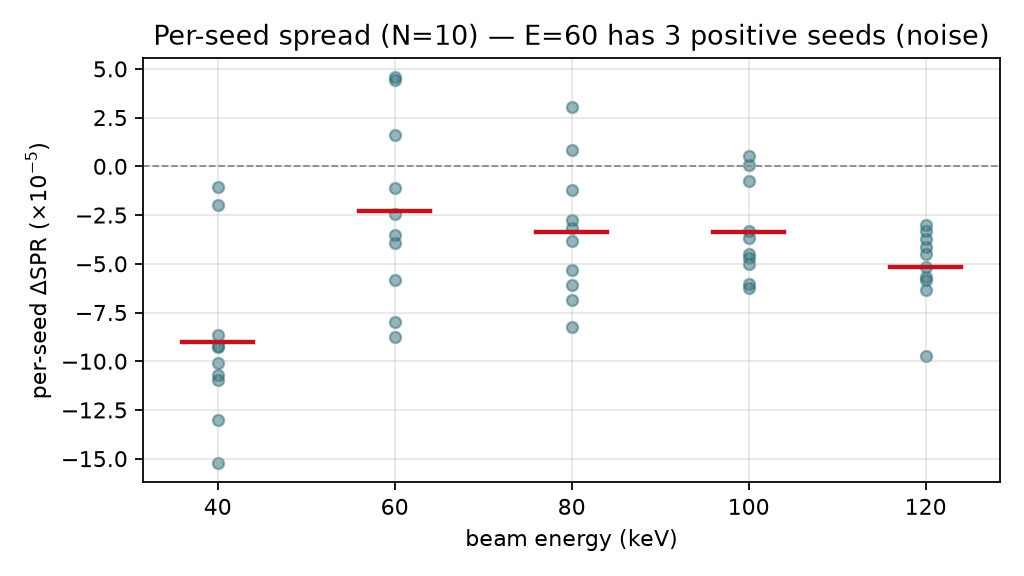
\includegraphics[width=0.62\textwidth]{fig_cl3/perseed.png}
\caption{การกระจายของ $\Delta$SPR ต่อ seed ($N=10$); เส้นแดง = ค่าเฉลี่ย. $E=60$ มี seeds เป็นบวก 3 ตัว
(noise) ทำให้ประเมินอ่อนกว่าจริง}
\end{figure}

\subsection{การวิเคราะห์ within-seed (repeated-measures) --- ยืนยันการเสริมที่พลังงานต่ำ}
เนื่องจากทุกพลังงานใช้เมล็ดสุ่มชุดเดียวกันต่อ index (common random numbers) การวิเคราะห์แบบ \textbf{within-seed}
จึงตัดความแปรปรวนระหว่าง seed ออกได้ (power สูงกว่า between-seed มาก) --- เปรียบเทียบ $\Delta$SPR ที่ $E=40$
กับ $E\ge80$ \textbf{จับคู่ต่อ seed}: $9$ จาก $10$ seeds ให้สัญญาณที่ 40~keV แรงกว่า, $t=-4.24$,
\textbf{$p=0.0022$} $\Rightarrow$ \textbf{การเสริมสัญญาณที่พลังงานต่ำมีนัยสำคัญ} (ยืนยันกลไก photoelectric);
within-seed slope ของ $\Delta$SPR เทียบ $E$ ให้ one-sided $p=0.038$ (สัญญาณอ่อนลงเมื่อ $E$ สูง)

\begin{figure}[h]\centering
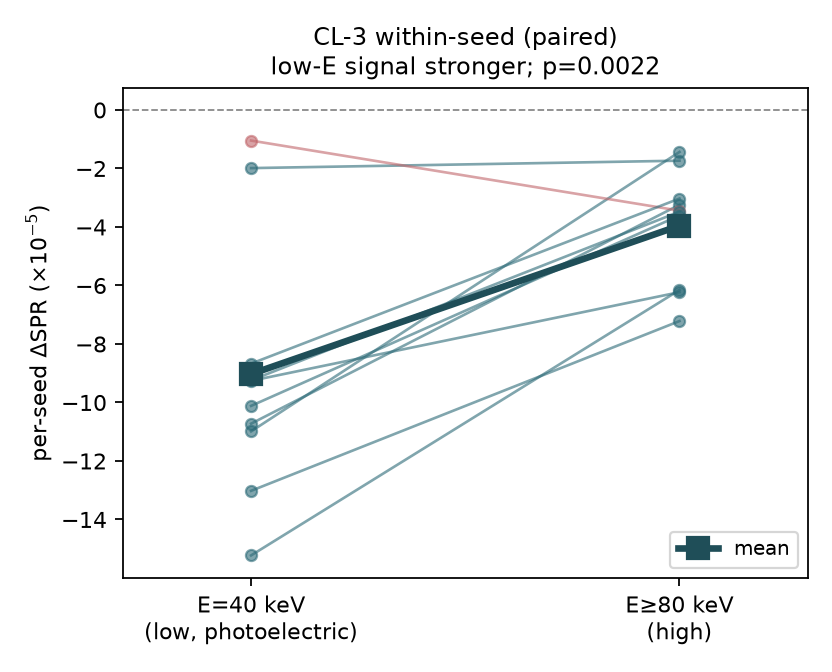
\includegraphics[width=0.48\textwidth]{fig_cl3/withinseed.png}
\caption{CL-3 within-seed paired: 9/10 seeds ให้สัญญาณที่ 40~keV แรงกว่า $E\ge80$ ($p=0.0022$) ---
เส้นน้ำเงินหนา = ค่าเฉลี่ย}
\end{figure}

\section{สรุปการทดสอบสมมติฐาน CL-3}
\begin{keybox}
\textbf{กลไกเชิงพลังงาน:}\ \textcolor{ok}{$\boxtimes$ \textbf{มีนัยสำคัญ (การเสริมที่พลังงานต่ำ)}}\\[4pt]
หลักฐานสามอย่างที่สอดคล้องกับฟิสิกส์ของการลดทอนในกระดูก: (1)~\textbf{สัญญาณแรงสุดที่ 40~keV} ---
\textbf{within-seed paired $E{=}40$ vs $E{\ge}80$: $p=0.0022$} (9/10 seeds) และ between-seed $p=0.0001$;
(2)~\textbf{baseline SPR ลดลง monotonic} ($\rho=-1.00$, $p<0.001$); (3)~ตาม photoelectric
($\mu_{\text{bone}}\propto1/E^3$) $\Rightarrow$ สัญญาณ\textbf{ผูกกับฟิสิกส์การลดทอน มิใช่ artifact เชิงตัวเลข}.
ข้อจำกัดที่เหลือ: การประเมินราย\textbf{พลังงานเดี่ยว} 60--120~keV ยัง noisy ที่ $N=10$ (เช่น $E=60$, $p=0.16$)
--- แต่\textbf{กลไกโดยรวมมีนัยสำคัญ}
\end{keybox}

\section{การตีความและงานถัดไป}
\begin{itemize}
  \item \textbf{ฟิสิกส์:} การเสริมที่พลังงานต่ำ + baseline ที่ลดลง สอดคล้องกับ $\mu_{\text{bone}}(E)$ ที่ photoelectric
        ครอบงำใต้ $\sim$50~keV แล้วเข้าสู่ Compton regime ที่แบนกว่า --- เป็น ``ลายเซ็นเชิงพลังงาน'' ที่ artifact
        เชิงตัวเลขเลียนแบบได้ยาก
  \item \textbf{นัยเชิงประยุกต์:} การถ่ายภาพที่\textbf{พลังงานต่ำ}เพิ่มความไวต่อรอยแตก (แลกกับ dose ที่สูงขึ้น)
        --- จุดที่ควรศึกษาต่อในเชิง optimization
  \item \textbf{งานถัดไป (เลือกได้):} กลไกยืนยันแล้วด้วย within-seed; หากต้องการเส้นโค้ง $|\Delta\mathrm{SPR}|(E)$
        เชิงปริมาณราย\textbf{พลังงานเดี่ยว}ที่คมชัด ให้รันซ้ำ \code{n_seeds=20--30}; พิจารณาแยก primary/scatter
        เพื่อดูองค์ประกอบเชิงพลังงาน
\end{itemize}

\vfill
\noindent{\color{theme!45}\rule{\textwidth}{0.4pt}}\\
{\small\color{ink} รายงานเฉพาะ CL-3 ประกอบ \code{report/methodology.pdf}. ข้อมูล: 5 พลังงาน $\times$ 10 seeds
(0.54~มม.). ดูรายงานอื่นที่ \code{report/} และ https://wwaxray.baanwit.com/doc/report/}

\end{document}
